% F26 Image comparison on a stage photo: Student vs the original Multi-HMR-Anny. Added 6 Nov.
% Image: slide 11 of the author's final presentation (5 Nov), ppt/media/image16.png (2016 x 736, three 672-px panels),
% produced by demo_image_compare.py (docs/image_comparison.md: FOV 55 degrees along the longer side, panel size 672);
% black letterbox bars cut (scratchpad script make_images.py), labels unchanged. Saved as figures/img/F26_image_compare.jpg
% (2016 px wide, JPEG quality 85). 12 Nov revision: the three 672-px panels are shown as 1 + 2 at half text width
% (trim in bp = px at 72 dpi), so that the two model panels are larger. "3 visible detection(s)" per model = the panel labels.
\begin{figure}[!tbp]
\centering
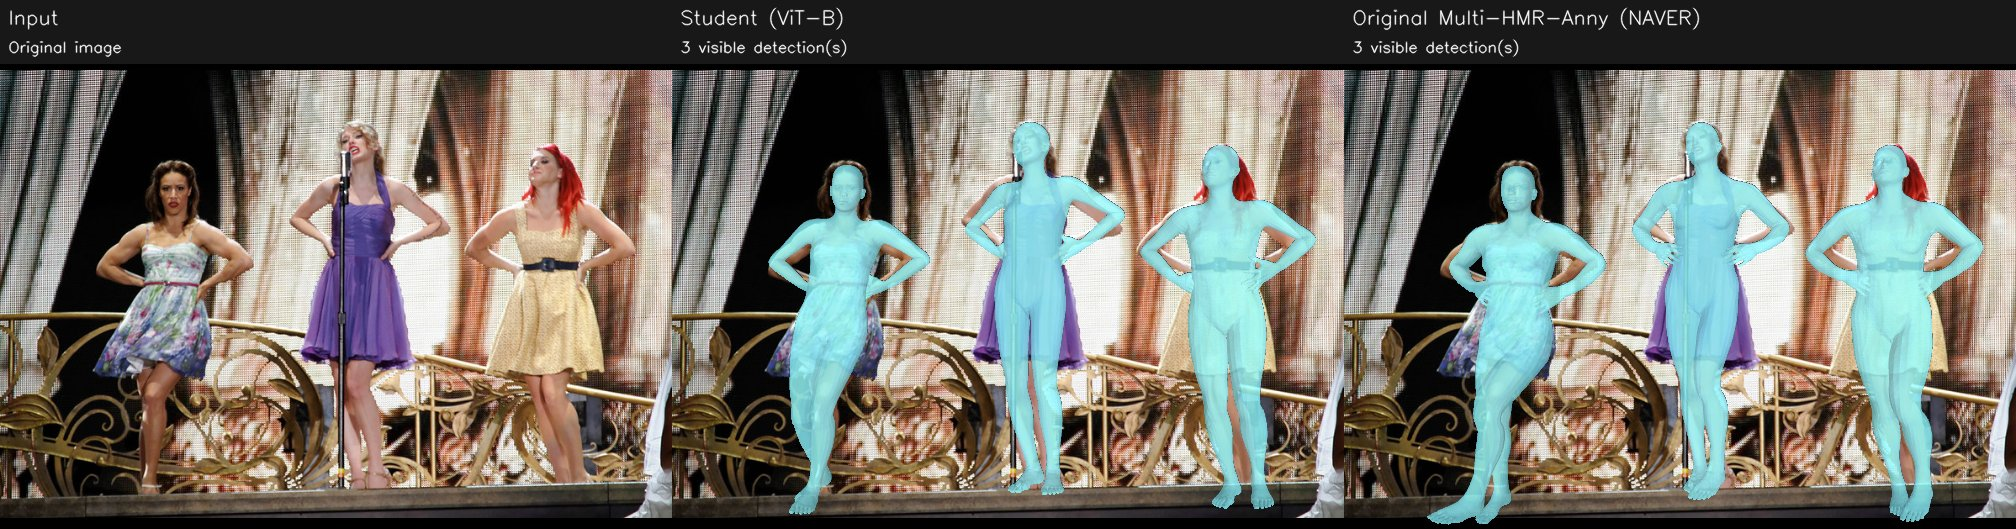
\includegraphics[width=0.49\linewidth, trim=0 0 1344 0, clip]{F26_image_compare.jpg}\\[3pt]
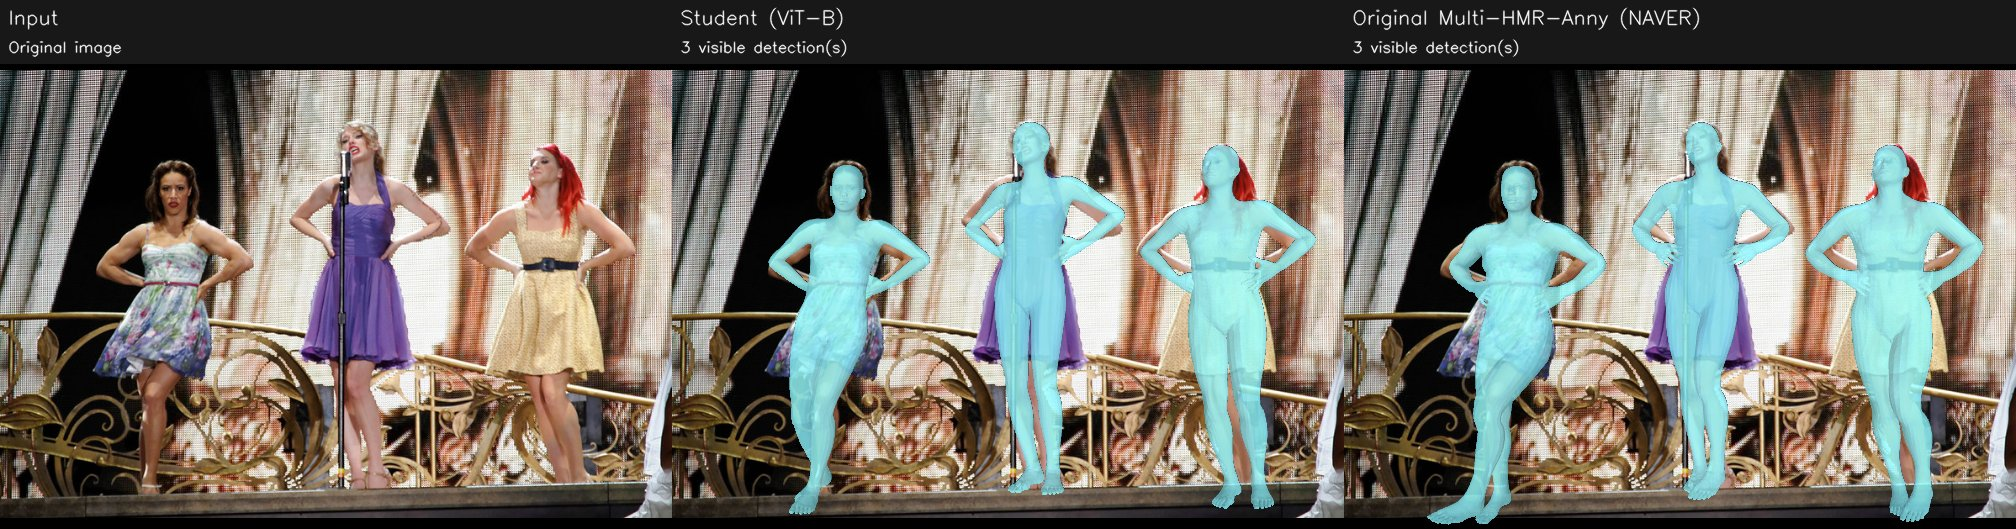
\includegraphics[width=0.49\linewidth, trim=672 0 672 0, clip]{F26_image_compare.jpg}\hfill
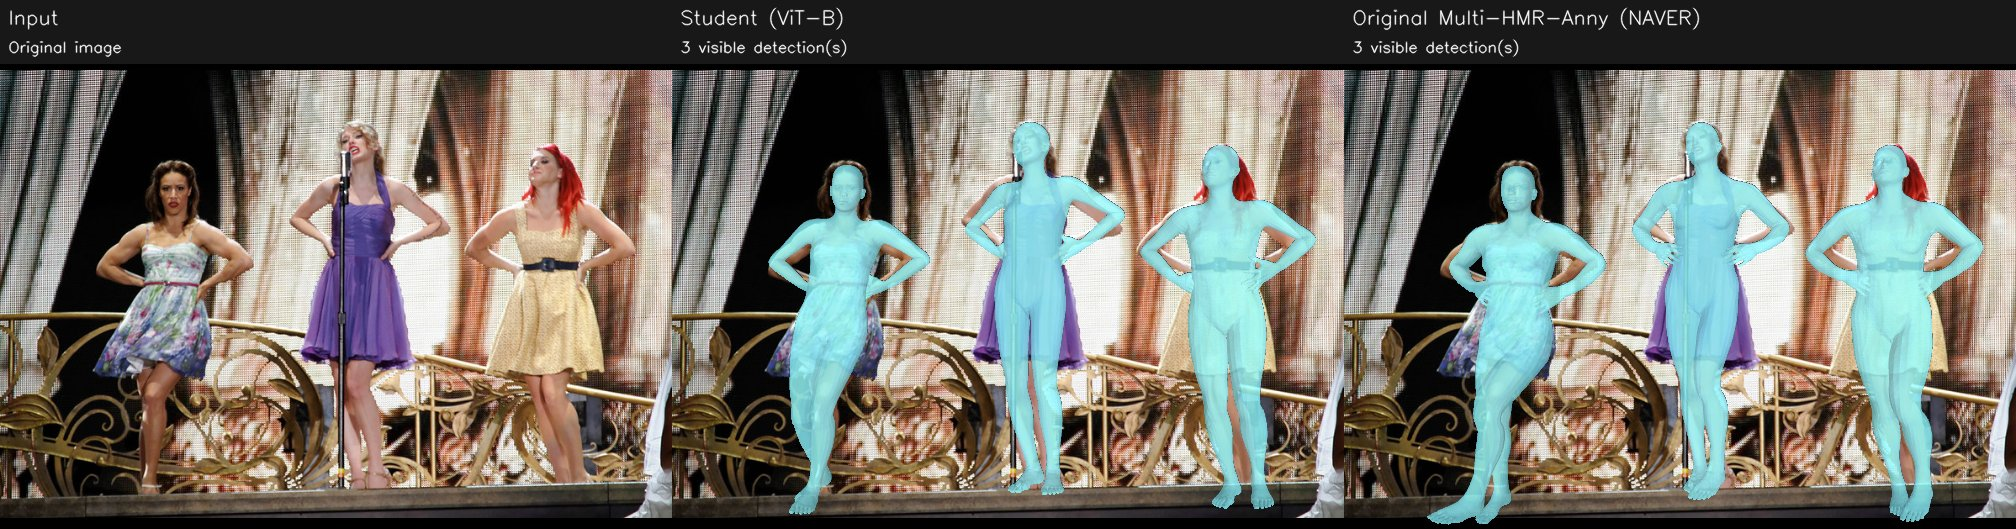
\includegraphics[width=0.49\linewidth, trim=1344 0 0 0, clip]{F26_image_compare.jpg}
\caption[Image comparison: student and released baseline]{A real photograph of three people on a stage: input
(top), the student (bottom left, labelled ``Student (ViT-B)'') and the released baseline (bottom right, labelled
``Original Multi-HMR-Anny (NAVER)''). Both models detect all \ImageCompareDetections{} people; the photograph has no
ground truth.}
\label{fig:image-compare}
\end{figure}
